\chapter{Knihovny použité při sestavování programu Sound Analyzer}
\label{kap:libraries}

V této kapitole vám přiblížím knihovny použité na projektu \emph{Sound Analyzer}.
Základem všech je ovšem stadardní knihovna jayka \emph{C++}.

\section{Knihovna openCL}
\label{kap:opencl}

Tato kapitola je výtahem z dokumentace k openCL (\cite{opencl}).
Úplnou dokumentaci lze najít \url{kronos.org}.

\subsection{OpenCL framework}

OpenCL \emph{framework} obsahuje tři hlavní části:

\begin{itemize}
\item OpenCL platformní vrstva -- dovoluje \emph{hostiteli} zjišťovat možnosti \emph{zařízení}, a~vytváří \emph{kontext}.
\item OpenCL runtime -- všechny operace manipulující s~kontextem.
\item Překladač openCL -- vytváří spustitelné objekty obsahující \emph{jádra}. Vychází z  ISO C99.
\end{itemize}

\subsection{Architektura openCL}

OpenCL je průmyslový standard pro programování heterogenních skupin CPU, GPU a~dalších zařízení organizovaných do jedné platformy. Je to více než jen jazyk.
Je to celý framework  který obsahuje programovací jazyk, API,
knihovny a~runtime systém pro podporu vývoje. OpenCL poskytuje nízkoúrovňovou
abstrakci hardware plus framework.
\\
V dalších kapitolách blíže popíši následující modely:
\begin{itemize}
\item Model platformy.
\item Model paměťový.
\item Model prováděcí.
\item Model programovací.
\end{itemize}

\subsection{Diagram tříd}

Obrázek (viz obr. \ref{obr:openclclassdiagram}) popisuje specifikaci openCL jako UML diagram tříd.
Jsou na~něm znázorněny jen základní třídy, nikoli jejich atributy.

\begin{figure}
  \begin{center}
    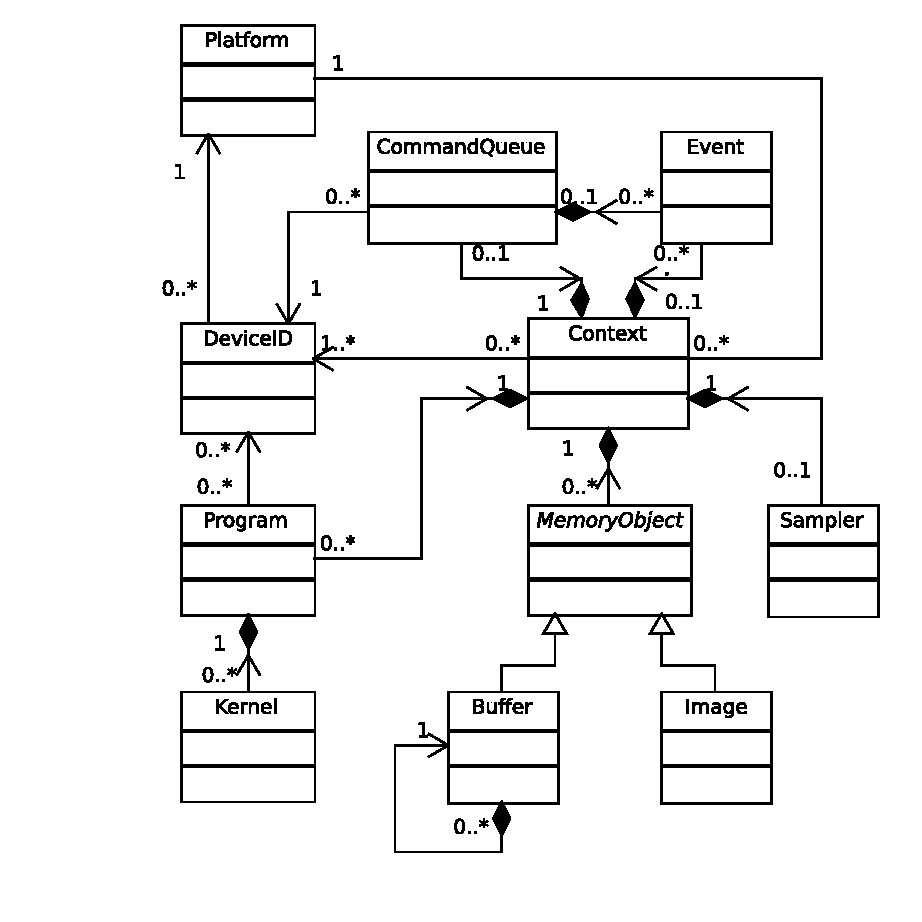
\includegraphics[scale=1]{obr/ClassDiagram}
  \end{center}
  \caption{UML Diagram tříd}
  \label{obr:openclclassdiagram}
\end{figure}

\subsection{Model platformy}

Model se sestává z \emph{hostitele}  připojeného k jednomu nebo více
openCL \emph{zařízením} . Toto  \emph{zařízení} je dále děleno
na~jednu nebo více \emph{výpočetních jednotek}  a~tyto
\emph{výpočetní jednotky} jsou dále děleny na~jednu nebo více \emph{zpracujících
jednotek} .

OpenCL \emph{aplikace}  běží na~\emph{hostiteli} 
OpenCL \emph{aplikace} posílá \emph{příkazy}  z \emph{hostitele}
ke zpracování výpočtů do \emph{zpracujících jednotek} 
v rámci \emph{zařízení}. \emph{Zpracující jednotky} v~rámci \emph{výpočetní jednotky}  provádějí jednu  sadu instrukcí jako \emph{SIMD} 
 jednotky, nebo jako \emph{SPMD}  jednotky, kde každá
\emph{zpracující jednotka} má svůj čítač instrukcí.

\subsubsection{Podpora různých verzí}

OpenCL je navrženo s~podporou více \emph{zařízení} s~různými možnostmi společně provozovanými pod jedním \emph{hostitelem}. To ovšem znamená, že každé zařízení může splňovat jinou verzi knihovny openCL. Máme tedy verzi runtime prostředí a~zvlášť verzi u~každého \emph{zařízení}. Dále každé \emph{zařízení} může podporovat svou vlastní verzi
jazyka openCL~C.


\subsection{Prováděcí model}

Když je \emph{jádro} pověřeno \emph{hostitelem} k provedení, je třeba definovat indexový prostor. Instance \emph{jádra}  se nazývá \emph{pracovní položka}  a~je definována bodem v~indexovém prostoru, který definuje \emph{globální ID}  pro tuto \emph{pracovní položku}. Pracovní položka je svázánu s jedním, konkrétním jádrem výpočetního zařízení.\emph{Pracovní položky}
jsou organizovány v~ \emph{pracovních skupinách} .
\emph{Pracovní skupiny} mají unikání ID \emph{pracovní skupiny}. \emph{Pracovní položky} můžeme v~indexovém prostoru identifikovat stejným způsobem, Také mají své \emph{globální ID}. Mimo to je ale můžeme identifikovat dvojicí \emph{globální ID} \emph{pracovní skupiny} a~\emph{lokálním ID} (v rámci této \emph{pracovní skupiny}).
\\
Indexový prostor, který je definován knihovnou openCL, je $N$-rozměrná pole. Nazývají se \emph{NDRange}. $N$ může být jedna, dvě nebo tři. To znamená, že i indexy jsou $N$-prvkové. Položky indexu začínají vždy od nuly.
\\
Index tedy definuje určitou \emph{pracovní skupinu} v~rámci \emph{výpočetní jednotky}. Stejným způsobem je také definován index \emph{pracovní položky} v~rámci \emph{pracovní skupiny}.

\subsubsection{Kontext a~fronty příkazů}	

\emph{Kontext}  vytváří a~spravuje \emph{hostitel} prostřednicvím funkčních volání openCL API. \emph{Hostitel} v~\emph{kontextu} vytvoří zejména \emph{frontu příkazů} , aby mohl zařízení ovládat. Do těchto \emph{front příkazů} zapisuje \emph{příkazy} k provedení. Mezi tyto \emph{příkazy} patří:

\begin{itemize}
\item Příkazy k provádění jádra.
\item Příkazy pro práci s~pamětí.
\item Synchronizační příkazy.
\end{itemize}


V jednom \emph{kontextu} může být více \emph{front příkazů} které jsou prováděny nezávisle na~sobě.


\subsection{Paměťový model}

\emph{Pracovní položky} rozlišují čtyři druhy pamětí:

\begin{itemize}
\item Globální paměť.
\item Paměť konstant.
\item Lokální paměť.
\item Soukromá paměť.
\end{itemize}


\begin{table}[htbp]
\centering
 
\begin{tabular}{|c||c|c|c|c|}
\hline
Přístup z& \bfseries Global & \bfseries Constant & \bfseries Local & \bfseries Private \\
\hline
\hline
\multirow{5}{*}{\bfseries Hosta}  & Dynamická & Dynamická & Dynamická & Bez\\
& alokace & alokace & alokace & alokace\\
& & & &\\
& Přístup pro & Přístup pro & Není & Není\\
& čtení / zápis & čtení / zápis & přístup & přístup\\
\hline
\multirow{5}{*}{\bfseries Jádra}  & Není & Statická & Statická & Statická\\
& alokace & alokace & alokace & alokace\\
& & & &\\
& Přístup pro & Přístup pro & Přístup pro & Přístup pro\\
& čtení / zápis & jen čtení & čtení / zápis & čtení / zápis\\
\hline
\end{tabular}
\caption{Typy pamětí v~openCL}
\label{tab:typypameti} 
\end{table}

\emph{Aplikace} běžící na~\emph{hostiteli} vytváří \emph{paměťové objekty} v~{globální paměti}.


Paměť \emph{hostitele} a~\emph{zařízení} jsou na~sobě nezávislé. Nicméně je potřeba aby \emph{zařízení}
a~\emph{hostitel} spolu nějakým způsobem komunikovaly.
Toho je docíleno kopírováním paměti nebo jejím sdílením. Kopírování může býti jak blokující,
tak neblokující. Blokující nebo neblokující může být
rovněž mapování paměti. \emph{Aplikace} většinou
mapuje paměť na~nezbytně nutnou dobu a~když jsou všechny operace čtení a~zápisu dokončeny, opět
paměť odmapuje.

\subsection{Programovací model}

OpenCL nabízí dva programovací modely, respektive dva základní přístupy. \textbf{Datově paralelní model} a~\textbf{úlohově paralelní model}.

\subsubsection{Datově paralelní model}

V datově paralelním programovacím modelu provádějí všechny \emph{pracovní položky} v~rámci \emph{pracovní skupiny} současně jednu sadu instrukcí. Model je rozdělen na~dvě kategorie.
U \textbf{explicitní} definuje aplikace, jak bude \emph{pracovní skupina} rozdělena na~\emph{pracovní položky}. U \textbf{implicitní} aplikace pouze definuje, kolik pracovních položek chce použít a~rozdělení \emph{pracovní skupiny} na~\emph{pracovní položky} nechá na~knihovně openCL.

\subsubsection{Úlohově paralelní model} 

V úlohově paralelním modelu je každé \emph{jádro}\ref{sec:kernel} vykonáváno zcela nezávisle na~jiných. Znamená to, že je prováděno v~\emph{pracovní skupině}, která má jednu jedinou \emph{pracovní položku}. V~tomto modelu je zdůrazněna paralelnost:

\begin{itemize}
\item používáním vektorových datových typů.
\item řízením více úloh.
\end{itemize}

\subsubsection{Synchronizace}

\emph{Pracovní položky} položky mohou být synchronizovány mezi sebou využitím \emph{bariér}. Pro synchronizaci \emph{pracovních skupin} mezi sebou, žádný takový mechanismus neexistuje.

\emph{Příkazy} mají také možnost používat \emph{bariéry}. Tyto \emph{bariéry} zajistí, že všechny příkazy zařazené před touto \emph{bariérou} ve \emph{frontě příkazů}, budou provedeny dříve, než se začne s~prováděním dalších \emph{příkazů}.

Všechny \emph{příkazy} \emph{hostitele}, které  vkládají \emph{příkazy} do \emph{fronty příkazů}, vracejí objekt \textbf{události}. Další \emph{příkaz} ve \emph{frontě příkazů} může na~tuto událost čekat.

\subsection{Paměťové objekty}

Jsou dvě kategorie \emph{paměťových objektů}: \emph{obrázky}  a~\emph{buffery} .
\emph{Buffer} je řada objektů nějakého typu a~můžeme k nim přistupovat pomocí rukojeti (handle \ref{sec:handle}). Naproti tomu je struktura \emph{obrázku} skryta a~k \emph{obrázku} můžeme přistupovat pouze pomocí speciálních funkcí jádra. \emph{Obrázek} nemusí mít stejný formát u \emph{hostitele} a~uvnitř \emph{jádra}.



